\chapter{How to Build a Fictional World --- Kate Messner}

Messner は、方法論的に正しいことを最初に行う。worldbuilding の definition から始めない。すでに働いている worlds から始めるのである。Gandalf は死んで戻ってくることができる。Matrix では、skill を download できる。Cheshire Cat は自分の head を juggle できる。Quidditch match は Golden Snitch が caught されるまで終わらない。ultimate question への answer は \(42\) である。こうした remembered laws の parade のあとでようやく、彼女はそれらを together に hold しているものを tell する。fictional world が memorable なのは、anything whatever を permit するからではなく、それが permit するものが stable rules に governed されているからなのだ。そこから講義は clean な sequence で unfold する。examples、principle、ordinary reality との contrast、book-world に対する reader の grasp、marks on a page がどうやって lived experience になるのかという deeper な puzzle、そして最後に、writer が world を build し、そこから story を emerge させる practical な method へと進む。

\section{まず examples から: rules をもつ worlds}

講義の opening は cumulative である。それぞれの example は、strange なものが persuasive になるのは、それが regular であるときだけだという reminder になっている。Gandalf の body は mortal で、その spirit は immortal である。Matrix には accelerated competence の mechanism がある。Cheshire Cat の logic は absurd だが、formless ではない。Quidditch には explicit な terminal condition がある。Douglas Adams の \(42\) でさえ、questions と answers が私たちの own rules には従わない world の lawful output のように sound するからこそ force を持つ。

冒頭を compact な note-form で record すれば、
\begin{align}
\text{mortal body} + \text{immortal spirit} &\Rightarrow \text{Gandalf can die and return},\\
\text{link up} + \text{hack code} &\Rightarrow \text{learn helicopter flight in seconds},\\
\text{Snitch caught} &\iff \text{Quidditch match ends},\\
\text{ultimate answer} &= 42.
\end{align}
となる。これらは、strict な mathematical sense における equations ではない。local な rule-statements である。だが Messner の point は、readers はこうした rules を通して worlds を remember する、ということだ。marvel は、form を持つがゆえに legible になる。

これによって講義は、最初の explicit な abstraction を行うことができる。
\begin{equation}
\text{consistent rules} \Rightarrow \text{believability} + \text{comprehensibility} + \text{explorability}.
\end{equation}
mere に surprising な world は thin である。ひとつの event が、次の event をどう読むかを教えてくれるとき、world は explorable になる。したがって講義が examples から始まるのは、本当の argument の前に私たちを entertain するためではない。本当の argument を visible にするためなのである。

\subsection{Question \& Answer}

\paragraph{Question.} invented world を random ではなく coherent に feel させるものは何か。

\paragraph{Answer.} その wonders が constrained されていることである。reader が、その world が何を allow し、何を forbid し、何を repeat するのかを infer できるようになると、world は novelties の pile であることをやめ、structure をもつ domain になる。

\section{real laws、page laws、そして authors が実際に build するもの}

そこから Messner は、より sharp な comparison を行う。gravity は、Harry Potter books を私たちの world の shelves に hold している。これは true だと私たちは know している。だが fiction の pages の上では、wizarding domain が once established されたなら、gravity は modified され、suspended され、あるいは別の rule に answered されうる。decisive な distinction は、law と lawlessness のあいだにあるのではない。一つの lawful domain と、別の lawful domain のあいだにあるのである。

Messner の phrase である ``a spectrum of physical and societal rules'' の useful な compression は、次のようなものだ。

\begin{definition}
fictional world は、図式的には
\begin{equation}
W = (R_{\mathrm{phys}},\,R_{\mathrm{soc}}),
\end{equation}
と要約できる。ここで \(W\) は world、\(R_{\mathrm{phys}}\) はその physical rules、\(R_{\mathrm{soc}}\) はその social rules である。これは note-writer の notation であって、lecture 由来の notation ではないが、lecture の actual structure を capture している。
\end{definition}

すると gravity の contrast は、慎重に言えば、
\begin{equation}
g_{\text{real world}} \neq g_{\text{wizarding page-world}}.
\end{equation}
と書ける。この shorthand の point は、Messner が physics を doing しているふりをすることではない。彼女の prose がすでに doing していること、すなわち reader の world の law と、book の内部の world の law とを distinguish していることを precise にすることにある。

だからこそ彼女は、ただちに scale を enlarge できる。science fiction や fantasy の authors は、mere な backdrop を choose しているのではない。intelligibility の whole infrastructure を build しているのである。
\begin{equation}
\text{rules} \to \text{maps} \to \text{lineages} \to \text{languages} \to \text{cultures} \to \text{universes}.
\end{equation}
これらの arrows は、articulated structure の increase を mark している。ひとつの altered law は、ひとつの trick を与える。laws、histories、institutions の connected system は、ひとつの world を与える。この時点で講義は、worlds とは何かだけでなく、それが readers に何をするのかを問う準備ができている。

\section{reader が book-world を understand するとき}

Messner の次の claim は、この講義の最初の major payoff である。worldbuilding がうまく done されると、reader は fictional world とその rules を、characters と同じくらいよく、そしてときには、book の外側の world を understand しているよりもよく understand できる。これは side remark ではない。講義の central tension を create する proposition なのである。もしそれが起こりうるなら、私たちは次に how を問わなければならない。

compact な note-form comparison としては、次のように書ける。
\begin{equation}
\text{reader's grasp of book-world} \gtrsim \text{reader's grasp of outside world}.
\end{equation}
この symbol \(\gtrsim\) は、Messner の phrase である ``just as well or even better'' の shorthand にすぎない。spoken lecture notation ではない。だが、この claim の strength を視界に保ってくれる。

講義の中で validated された唯一の image は、まさにここで useful である。それは equation ではない。spatial な contrast である。reader と open book が foreground を occupy し、small な story-world が pages から rise し、outside world が behind に separate な social field として現れる。この image は、その sentence が意味していることを示している。book の中の world は、しばらくのあいだ、より readable な domain になりうるのである。

\begin{figure}[h]
\centering

\includegraphics[width=0.82\textwidth]{lecture_09_figure_03.png}
\caption{reader、book-world、そして book の outside world。}
\end{figure}

screenshot は symbolic ではなく rhetorical なので、そのそばに cleaned な schematic を置くのが助けになる。screenshot は evidence として保ち、TikZ の redraw は interpretation として置く。

\begin{figure}[h]
\centering
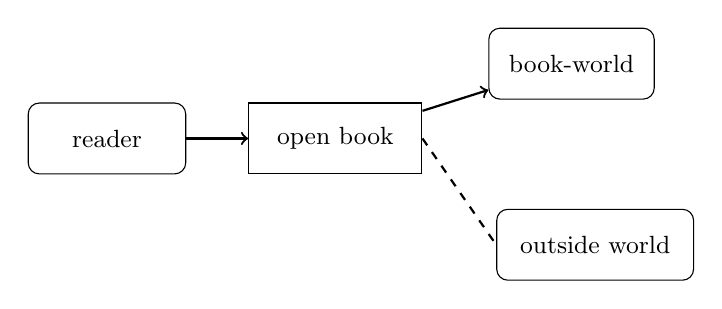
\begin{tikzpicture}[x=1cm,y=1cm]
\node[draw, rounded corners, minimum width=2.0cm, minimum height=0.9cm] (reader) at (0,0) {\small reader};
\node[draw, minimum width=2.2cm, minimum height=0.9cm] (book) at (2.9,0) {\small open book};
\node[draw, rounded corners, minimum width=2.1cm, minimum height=0.9cm] (inside) at (5.9,0.95) {\small book-world};
\node[draw, rounded corners, minimum width=2.5cm, minimum height=0.9cm] (outside) at (6.2,-1.35) {\small outside world};
\draw[->, thick] (reader) -- (book);
\draw[->, thick] (book) -- (inside);
\draw[dashed, thick] (book.east) -- (outside.west);
\end{tikzpicture}
\caption{book の中の world と、その outside world との contrast を示す、講義の schematic reconstruction。}
\end{figure}

この redraw の exact geometry は重要ではない。重要なのは講義の intuition である。reading は、ordinary life の rules よりも私たちに available な rules をもつ domain を produce しうるのだ。

\subsection{Question \& Answer}

\paragraph{Question.} どうして book-world は reality よりも legible になりうるのか。

\paragraph{Answer.} book-world は intelligibility のために structured されているからである。その rules は chosen され、repeated され、mutually supporting になるように作られている。reality のほうが richer ではあるが、同時に noisier でもある。講義の point は、よく built された fictional world は、したがって reader にとって、より tractable な system になりうるということだ。

\section{しかし、どうやって? ぐにゃぐにゃの marks が worlds になるまで}

まさにこの point で Messner は、forward movement を stop し、講義最大の question を ask する。だが、どうやって? page 上の squiggles がどうやって eye へ light を reflect し、brain へ signals を送り、それが narrative として decode され、emotionally に私たちを動かし、そして最後には、last mark が read されたあとで world に戻る私たちの way を alter するのか。

講義自身の chain は、compact には
\begin{equation}
\text{squiggles on page} \to \text{signals to the brain} \to \text{decoded narrative} \to \text{emotion/thought/action} \to \text{changed perspective}.
\end{equation}
と書ける。ここでは、lecture の rhythm を preserve すべきである。Messner は matter を information transfer alone に reduce しない。彼女は、chain を perception から feeling へ、feeling から action へ、action から altered perspective へと、明示的に widen している。reading の end は mere comprehension ではない。どれほど small であれ、transformation なのである。

\paragraph{Worked derivation.} steps へ unpack すると、lecture の mechanism は次のようになる。
\begin{enumerate}
\item marks が page に置かれる。
\item page から reflected した light が eyes に届く。
\item nervous system がその input を signals に convert する。
\item mind が patterned signals を narrative として decode する。
\item narrative が emotion、thought、imagination を recruit する。
\item reader は fictional world に lived domain として enter する。
\item book を leave したあとで、reader の ordinary world の view は different になっているかもしれない。
\end{enumerate}

これは、functional derivation であって、finished な science of reading ではない。Messner はその点に careful である。彼女は explicitly に、誰かが fully に答えを know しているとは思えない、と言う。この concession は重要である。講義は、その mystery を solve したふりをして craft へ急ぐことをしない。mystery を mystery のまま立たせ、それでも practice のほうへ向きを変えるのである。

\subsection{Question \& Answer}

\paragraph{Question.} page 上の marks は、どうやって reader の mind の中で lived world になるのか。

\paragraph{Answer.} 講義は theorem ではなく chain によって答える。marks は signals になり、signals は decoded order になり、decoded order は narrative になり、narrative は feeling を強く recruit して immersion と return を生む。exact な mechanism は partly obscure なままである。だが operative sequence は plain である。

\section{mystery から method へ}

lecture が mystery を立たせたところで、scale が変わる。fantastical worlds は毎日 created されている、と Messner は言う。私たちの minds の中で、computers の上で、さらには napkins の上でさえ。practical な premise は、imagination と、その imagination の内側に live する willingness があれば、begin するには enough だということだ。そこから講義は、writer の method へ descend していく。

最初の step は historical である。
\begin{equation}
\text{past events} \to \text{timeline} \to \text{present structure of the world}.
\end{equation}
これは、最初に見えるより強い claim である。私たちは decoration から begin するのではない。何が起こり、どんな order で起こり、どんな long consequences をもったのかを ask するところから begin する。したがって timeline は extra material ではない。world が現在のように arranged されているのはなぜか、という question に対する、最初の formal answer なのである。

そこから Messner は、ordered families of questions によって proceed する。macro scale では、law、power、belief、value を ask する。
\begin{equation}
(\text{rules},\ \text{government},\ \text{power},\ \text{beliefs},\ \text{values}).
\end{equation}
ordinary life の scale では、lived texture へ descend する。
\begin{equation}
(\text{weather},\ \text{home/work/school},\ \text{food},\ \text{play},\ \text{young/old},\ \text{plants/animals},\ \text{technology},\ \text{transportation},\ \text{communication},\ \text{information}).
\end{equation}
この ordering は pedagogically exact である。私たちは constitutive law から social structure へ move し、それからはじめて daily life へ向かう。world は、その slogans を know しただけではまだ inhabitable ではない。people が何を eat し、どう move し、何を fear し、何を teach し、何を punish し、朝にどんな weather に meet するのかが分かったときにはじめて、inhabitable になるのである。

\paragraph{Worked example.} Messner の method は、world-description に対する disciplined な update rule として書き換えることができる。
\begin{enumerate}
\item world の past を specify し、それを timeline として organize する。
\item どの physical rules と social rules が in force しているかを determine する。
\item 誰が govern し、誰が power を持ち、人々が何を believe しているかを ask する。
\item society が何を value し、violation をどう handle するかを ask する。
\item weather、work、school、food、play、age、ecology、technology といった daily realities へ descend する。
\item world が list であることをやめ、place になるまで続ける。
\end{enumerate}
lecture が求めているのは exhaustive な paperwork ではない。world が coherent に answer back し始めるだけの structured attention なのである。

\section{world から story へ}

終わりになってはじめて、Messner は lecture の real destination を reveal する。worldbuilding は endpoint ではない。story である。reader がそれを know することを私たちが hope するのと同じくらい world を know したなら、その inside に characters を set free にし、何が follows するかを ask する。すると world は background であることをやめ、causal なものになる。

Messner の closing compression は、
\begin{equation}
\text{world} + \text{characters} \Rightarrow \text{shaped individuals} \Rightarrow \text{conflict} \Rightarrow \text{story}.
\end{equation}
となる。この equation は最後に立てておくに値する。なぜなら、それがそれ以前の everything を reinterpret するからである。rules は、決して merely ornamental だったのではない。timeline は、決して merely archival だったのではない。questionnaire は、決して merely descriptive だったのではない。すべては pressure のための preparation だったのである。world は、それに inhabit する者たちが何を want しうるか、何を fear しうるか、何を violate しうるか、何になりうるか、したがってどんな kinds の conflict が appear しうるかを shape する。

もっと blunt に point を put することもできる。people を欠いた world は、ひとつの dossier を与える。world を欠いた people は、abstractions を与える。story は、structured な people が structured な world に meet し、その constraints の下で move することを forced されたときに始まるのである。

\subsection{Question \& Answer}

\paragraph{Question.} worldbuilding は、いつ background であることをやめ、story になり始めるのか。

\paragraph{Answer.} world の structure が choice を govern し始めたとき、それは story になる。characters が world の rules、values、technologies、punishments、permissions の下で live しなければならなくなると、conflict が appear する。その point で world は scenery ではない。drama の active terms の一つなのである。

\section{まとめ}

Messner の lecture は、fictional worlds についての compact だが genuine な mathematics を与えてくれる。strong な invented worlds は rule-governed である。その laws は ordinary life の laws と sharply に differ していてよい。だが、その difference 自体が coherent でなければならない。construction が succeed すると、readers は book の internal world を驚くほど clear に learn できる。この fact は、page 上の marks がどうやって lived experience になるのかという deeper な puzzle を raise する。そして lecture は、その puzzle を partly mysterious のまま leave する。だがそのあと、craft の level では practical な answer を与える。world の past を construct し、その laws と institutions を specify し、daily life へ descend し、それから resulting structure の内部で characters を move させるのだ。その moment に、worldbuilding は preparation であることをやめ、story になる。